\chapter{Methodology}
\label{Methodology}

\section{Introduction}
\label{Method:Intro}

In the previous chapter, I describe the recent shift toward a dementia lens that encompasses individuality, relationships, and supporting decision-making. In research that adopts relational approaches, researchers have designed approaches that use creativity and longer-term engagements to build relationships between the researcher and the participant. From here, I review literature outside the HCI space to respond to missing gaps in the HCI literature which focuses on ethical dilemmas, public perception, and ways to adapt methodological approaches to be more inclusive for later stages of dementia. Finally, I conclude the literature by providing a set of avenues of investigation that might broaden our understanding of designing and developing technology for and with people with dementia. These avenues are examined in the PhD.

In this chapter, I describe the methodological approach taken in the thesis that stretches across the data chapters. I begin the chapter by introducing the epistemological approach adopted in this thesis. Following, I describe the influence Participatory Design and co-design approaches have on the methodology \citep{duarte2018participatory}. The concluding sections of the methodology chapter discuss the ethical complexities of the methodology, data collection processes, qualitative data analysis method, and reflexive practice. This chapter closes by summarising the methodology for the thesis by returning to the research questions.  

\section{The social construct of dementia}
\label{social construct}
Through this thesis, I took a social constructionist approach to this research, in which the creation of knowledge is a collaborative process. Therefore, the way I structured the studies and interpreted the data is significantly influenced by my relationship with the participants and my understanding of dementia \citep{surr2006preservation}. Social constructionism argues that the self is formed through language and interactions of varying kinds that are equally important in defining the person's individuality \citep{sarup1996identity}. Further, given that the thesis focuses on the perspectives of diverse stakeholders involved in the design process, constructionism recognises that `multiple knowledges' exist together that shape and transform reality through social interactions and language \citep{mckeown2015you}.

As part of the changes that come with dementia, the social structures and roles can be disrupted \citep{hampson_dementia:_2016}. Challenges within previously familiar surroundings can cause issues for the person with dementia, who may feel less able to express and explore their identity \citep{john_killick_claire_craig_creativity_2012}. As we live in a society that places a high value on cognitive ability, a diagnosis of dementia can put significant strain on meaningful interactions, relationships, and activities. As a diagnosis continues to progress, the person with dementia and those around them must continuously learn to live with the changing roles and decline in abilities. For dementia, a social constructionist approach ensures the person with dementia is at the forefront of the design or care. Similarly, this view of dementia mirrors the work of \cite{kitwood1997dementia}, who draws attention to how we communicate with people with dementia, the person's cultural values, history, and the promotion of people with dementia being respected and engaged with their own care. With this in mind, not only can the sharing of lived experiences build a more positive construction of dementia, but the act of sharing and creating these stories can support the reclaiming of social identity \citep{ryan_dementia_2009}.

\section{User participation in the design process}
\label{ParticipationDesignProcess}

\begin{figure}[htp]
    \centering
    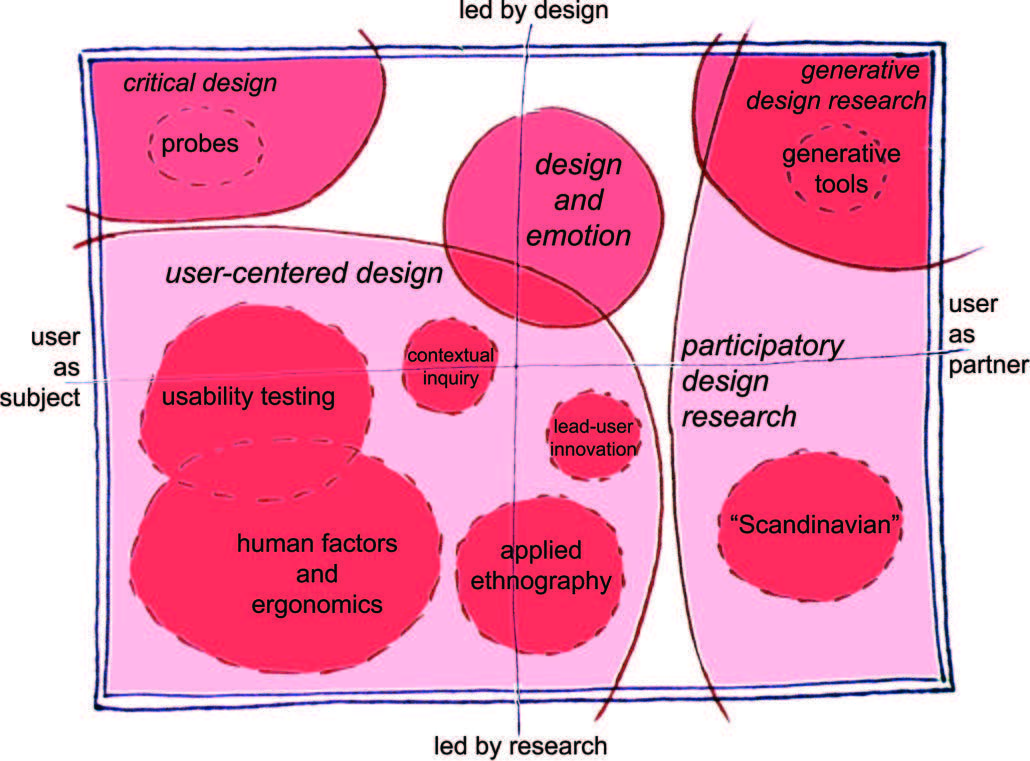
\includegraphics[width=0.6\linewidth]{Images/Methodology/Landscape_of_Design.jpg}
    \caption{Landscape of design research by  \citep{sanders2008co}}
    \label{fig:LandscapeOfDesign}
\end{figure}

Over the years, designers and researchers have moved towards design approaches that identify and involve users in the design process. In \cite{sanders2008co} work, the authors produced an overview of the landscape of human-centred design that shows the user's role and the research approach (seen in \ref{fig:LandscapeOfDesign}). For this thesis, my design approach seemingly moves between participatory design research and co-design. For participatory design, I take these approaches to \textit{``strive to learn the realities of the user's situation while the users strive to articulate their desired aims and learn appropriate technological means to obtain them''} \citep{simonsen2013routledge}. Additionally, for co-design, the approach recognises participants as experts of their experience who will work alongside designers in the design process - often through designers/researchers providing \textit{``appropriate tools for [participants] to express themselves''} \citep{sanders2008co}. In the following subsections, I dive into the use of participatory design and co-design.

\subsection{Participatory Design}
\label{Method:PD}
Participatory design (PD) has been influential in various social research fields, including HCI \citep{bannon2018introduction}. As the name implies, PD is about the \textit{design} of systems, products, or knowledge through \textit{participatory} methods to understand how users may interact or use an artefact or practice. These methods draw from ethnographic observations, interviews, focus groups, and qualitative content analysis. \cite{carroll2007participatory} articulate the importance of user participation from the following:

\begin{quote}
\textit{``The 'users' – that is, the people who stand to have their activity and experience transformed – ought to have a direct say and a meaningful role in how that comes to pass at the very least because they know a lot about what is precious and what is annoying in their current activity and experience, but equally because they are morally entitled to have a say in anything that might change everything.'' \citep{carroll2007participatory}    
}\end{quote}

Through these participatory approaches, PD aims to create a collaborative space between developers and the population group that was often separated from the design stages due to different experience levels \citep{duarte2018participatory}. Subsequently, PD has a significant political history where early PD work in the 70's \textit{``sought to rebalance power and agency among managers and workers''} \citep{bannon2018introduction}. Although PD has radically altered from what it was in the 70's, PD is still a popular approach to tackle communication barriers between different expertise levels. 
Within the general structure of PD, \cite{halskov2015diversity} argue they are five fundamental aspects of PD:
\begin{enumerate}
\item politics - \textit{``people who are affected by a decision should have an opportunity to influence it''}
\item People - \textit{``People play critical roles in design by being experts in their own lives''}
\item Context - \textit{``The use situation is the fundamental starting point for the design process''}
\item Methods - \textit{``Methods are means for users to gain influence in design processes''}
\item Product - \textit{``The goal of participation is to design alternatives, improving quality of life''}
\end{enumerate}

Halskov \& Hansen review highlights that HCI and other fields are diversifying and rethinking what participation may be within their domains, resulting in a highly diverse set of studies that reconfigure methods to fit the needs of participants to provide participation - particularly those who are considered marginalised, such as children, older adults and those who have varying cognitive deficits. For instance, \cite{spiel2018micro} conducted a series of PD studies with marginalised children that describe a set of ethical challenges of conducting PD within the space and the necessity to tailor participation for the children. The authors present detailed insights into tailoring PD processes to negotiate \textit{``what the children can do and the desires they have''}, design safe and attuned spaces \textit{``for the participation of children on their own terms''} and \textit{``make ethical judgments''} that are attuned to kindness and learning. Furthermore, \cite{vines_configuring_2013} describe several issues that PD needs to address. These challenges centre on the shared control and agency between researchers and participants. For instance, the author's highlight the need for transparency of participant and researcher's roles; how researchers present and analyse participants contributions; and further examine how participants can take agency of the design process and reinvent methods to suit their needs.

\subsection{Co-design}
\label{co-design}
Although co-design and participatory design approaches share the same values in user participation processes, co-design differs in creative acts of making. In co-design, the user's role \textit{``plays a large role in knowledge development, idea generation and concept development''} \citep{sanders2008co}. The researcher's role is to support sharing the participant's experience through design activities and tools for ideation. While creativity varies from participant to participant, the consensus of co-design is for the designer/researcher to generate and design ideas together with users, often being part of the design team as \textit{``expert[s] of their experiences''} \citep{visser2005contextmapping}.   

In co-design, participants can take part in multiple areas of technology development. For instance, designers may use scenarios and storyboards in the pre-design stages that provide space for discussion, reflection, and observation \citep{bell2019collaborative}. While at the evaluative stages of development, the research may take the form of a prototype where the system or product can be tested and ideated through participants' interactions and responses to how the prototype might fit into their everyday lives. Often, to upskill or provide participants with the ability to participate in the design processes, much work in co-design communication has been devoted to developing toolkits, cultural probes and prototypes to ensure participants express their ideas about technology and future uses \citep{medina_angarita_what_2020}. For instance, toolkits come in many different forms, from card games \citep{logler2018metaphor}, open-ended DIY resources \citep{meissner2018schnittmuster}, to interactive games to evoke creativity and learning \citep{ellis2021tapeblocks}, and the simplification of complex frameworks or algorithms to aid practitioner and public understanding \citep{krafft2021action}. Within this body of work, researchers have highlighted how the collaboration of expert curators and the application of adaptable co-design approaches are often necessary to design a practical toolkit within certain domains. 

For instance, \citep{krafft2021action} describes a yearlong process engaging with several partnering organisations, a team with diverse expertise, and a participatory action research approach for designing an Algorithmic Equity Toolkit. This toolkit was then comprised of definitions of AI, flowcharts, worksheets and probing questions to be posed to government agencies and policy-makers \citep{katell2020toward}. Critically, Lee and Singh argue some toolkits may be overbearing in terms of their information load and intended use, and raise a challenge for toolkits to be made \textit{``plug and play''}, within the designer or developer's workflow \citep{lee2021landscape}. While toolkits are only one of many approaches for generative stages in the design process, this work demonstrates the complexities and expertise for curating such resources to provide participants with engaging ways to participate in design. Further, \cite{hendriks_challenges_2014} examine how co-design tools may not be appropriate for people with dementia, especially when many methods require verbal or visual expressions. This is further complicated by involvement in earlier stages of development where creative thinking and conceptualisation are required, which I detail in the following section \ref{method:DementiaPD}.

As discussed above, both participatory design and co-design come with their set of challenges and distinct approaches to involve users in participation and curating participant-led technology. Throughout the studies in this thesis, each one provides insight into working with multiple stakeholders in various settings central to designing technology for people with dementia. As suggested by \cite{harrington_deconstructing_2019}, designing for marginalised populations often comes with complex, unforeseen tensions that require sensitive and personal consideration to provide collaborative engagement between the researcher and the marginalised community. Given that the following section describes adopting design approaches to provide meaningful and inclusive engagement, my overall approach is not tied to a specific participation approach. Still, it is influenced and shares many of the values that participatory approaches appropriate in design processes \citep{hansen2019participatory}.



\section{Reconstructing participatory design methods for people with dementia}
\label{method:DementiaPD}
By tradition, early design research in dementia has typically used focus groups, interviews, and the involvement of stakeholders who are `experts’ in the field, such as care partners, to make design decisions on behalf of people with dementia \citep{branco_personalised_2017}. However, as our understanding of dementia has changed over the years, so have our methods of involving and presenting the lived experiences of people with dementia. \cite{john_killick_claire_craig_creativity_2012} work in Creativity and Communication in Persons with Dementia, describe the importance of expression through the arts: 

\begin{quote}\textit{``Creativity is an expression of who we are, and when the arts form the vehicle or the means of channeling this creativity, the end result can embody something of the artist and their facets of personality'' \cite{john_killick_claire_craig_creativity_2012} pg.17}
\end{quote}

The authors highlight alternative ways that people with dementia can participate and express themselves, such as - laughing, music, writing, and painting. Similarly, \cite{kontos_presence_2015} research with Elder Clowns in long-term care facilities presents ways for people with dementia to produce language through other means than verbal communication. In the author's ethnographic account, the authors describe the playful interactions between residents and the clowns that offer moments of fantasy, laughter, and flexibility. The use of arts and humour gave residents \textit{``a sort of permission to behave in a way that conventional social and cultural codes might not sanction''}. Additionally, \cite{ryan_dementia_2009} draw on creative methods for communication and expression through writing as a way to reclaim identity, structure, and clarity on distinct thoughts and feelings. Consequently, writing projects a sense of self to loved ones, helping family members see past a relative's dementia and drawing attention to the creative potential for the person living with dementia. 

Likewise, some HCI research has expanded to explore how new technologies can attune to the creative wishes of people living with dementia. \cite{lazar_critical_2017} takes a critical dementia perspective to focus on how arts-based activities enable researchers to learn and draw from the experiences of people living with dementia. Taking part was noticed through \textit{``subtle shifts in gaze, facial expressions, and verbalisation''} and highlights the importance of tailoring the environment such as the brush, canvas and colours to fit the individual. The individuality in approach, suggests an enable for \textit{``connection between a person's `inner world' and `outer world' ''}, where individuals can express, reflect and process thoughts and ideas that come to them. \cite{stenhouse2013dangling} resonates with the above in engaging people with dementia in designing and creating their own digital stories. Through the participation, Stenhouse reports the necessary facilitation required in supporting people with dementia in the digital storytelling process. While this required facilitators to have knowledge of recording and narrating stories, the priority was building person-centred relationships with the participants to promote a safe space for sharing the stories. This embodied connection calls for methodologies that focus on bodily movement and action to learn from how people living with dementia configure their participation \citep{morrissey_creative_2015}.


\cite{lindsay_empathy_2012} adopted participatory design approaches for the early stages of dementia through workshops. The authors draw on the KITE approach that prioritises fostering an empathetic relationship between people with dementia and designers. Through this project, the authors share uncertainty about how their analysis of the data  \textit{``could, inadvertently, disempower the participants and undermine [their] relationship with [the] participant'' \citep[pg.528]{lindsay_empathy_2012}}. The authors stress how the deepening of the relationship between people with dementia and the designers has a knock-on effect where people with dementia are hesitant to critique designs for fear of offending one of the designers. Similarly, \cite{hendriks_challenges_2014} describes co-design's ethical and methodological complexities with people with dementia. While the author argues that participatory approaches have value in design work and can actively include people with dementia, the authors take the opportunity to report that there are several challenges that researchers may encounter during participation. For instance, participatory activities may be too stressful for participants and power relations can often be one-sided through researchers learning from participants and not vice-versa. Last, the authors state that participatory methods are challenging to translate to suit various stages of dementia.

From the work above, providing meaningful participation requires individualisation and personalised participatory approaches to fit the needs of people with dementia.  These practices include treating the person living with dementia as an individual in context; including the person living with dementia in research processes that aim to improve their quality of life; and acknowledging that dementia is a complex experience that often also includes social complexity, ageing and multi-morbidities, which require attuning to in design and research responses. In each data chapter, I describe each methodology in detail, which describes the reasons behind the approaches I made throughout the thesis. This consists of workshops, semi-structured interviews, hackathon events, online platforms and walking interviews. For this chapter, I describe the last two approaches as they are highly relevant to the section on `reconstructing participatory design methods for people with dementia':
\begin{enumerate}

\item \textbf{Participating in interviews}: describes the adaption of interviews as `walking-interviews' where people with dementia and families take the lead in the direction of the walking route and conversations
- seen in chapter four.

\item \textbf{Participating through online platforms}: describes the ways people with dementia are participating online through Twitter, blogs and online forums, which was an essential aspect of the participatory design approach implemented in the hackathon seen in chapter five and envisioning online participation on toolkit curation in chapter seven.
\end{enumerate}

\subsection{Participating in interviews}
\label{PD:Interviews}
In qualitative research, as an alternative to a rigid set of questions, researchers have adopted semi-structured interviews to adapt to the flow of the participant conversation \citep{cheston2000involving}. Semi-structured interviews offer flexibility from the interview guide where the opportunity to dive into people’s experiences, thoughts and ideas can be investigated in a more approachable way. However, this has drawbacks where the method is unlikely to provide comparisons between participant responses. Still, for working with researchers, people with dementia, designers and developers, it is a suitable interviewing procedure to explore complex everyday experiences  \citep{horton2004qualitative}. \cite{samsi2020interviewing} describe that by deviating from the interview questions, researchers can rephrase, adapt and move to alternative questions if the researcher feels the question is unnecessary or inappropriate within the setting providing a more comfortable and natural conversation for people with dementia.

However, while semi-structured approaches have been popular in dementia focused studies \citep{samsi_everyday_2013,mazaheri2013experiences,cheston2000involving,lejman2013ethics}, multiple researchers have adapted the process to fit the needs of people with dementia. For instance, \cite{mayer2013lessons} describe a series of guidelines to improve the comfortability and flow of the conversation. The authors suggest that using conversational probes that are based on memories or meaningful items can lift the conversation and keep choices and for the researcher to ensure design activities emphasise clarity and simplicity. In \citeauthor{suijkerbuijk_active_2019}'s systematic review, the author's highlight that the combination of interviews with observations is a popular approach when involving people with dementia in generative or evaluative phases of a study \citep{suijkerbuijk_active_2019}. In many person-centred approaches, researchers take an ethnographic or observational approach to move beyond interviews, where researchers explore the person with dementia's interactions in an everyday setting. This is often due to the challenge for later stages of dementia or those with verbal deficits in participating in interviews. For example, \cite{kontos_embodiment_2013} stress the need for creative ways to engage with the embodied and non-verbal through visual and sensory participatory methods. This work opens up our understanding of dementia where the \textit{``the body becomes a fundamental means of engaging with the world''} \citep[pg.296]{kontos_embodiment_2013}.

Another alternative methodology in social research that has gained popularity is walking interviews or `go-alongs' that provide meaningful engagements between the researcher and participants to deepen an understanding of lived experiences outside. \cite{hein2008mobile} argue's that sharing the `go-along' experience between the researcher and participants provides a richer data set during the interviewing and observation process. Further, as \cite{foley_struggle_2019} emphasises paying attention to the embodied interactions for those at later stages, \cite{kullberg2017walking}  discuss how walking interviews provide opportunities to explore the embodied interactions of people with dementia and that the approach puts less pressure on verbal communication. 

Following the person with dementia on the walk provides a sense of agency within the study where the location is on their terms. \cite{kullberg2017walking}  suggested that a walking interview approach provides a less stressful surrounding where participants may describe what they are seeing, how they are feeling, and even the potential for memories and experiences to be triggered by varying triggers from their senses. This is in contrast to research on 'wandering' and risk procedures for getting lost outside \citep{odzakovic2020verjoyed}. Further, \cite{brittain2017walking} stress that rather than reinforcing the 'aimless' wandering narrative of people with dementia, research should be challenging this by \textit{``highlight[ing] where it is that people wander''} which provides a more accurate perspective of people with dementia's abilities to guide and walk from A to B. With this in mind, using walking interviews to work with families with dementia provides data informed by experiences in the moment rather than solely relying on a participant's memory. Furthermore, providing activities instead of a sit-down interview promotes improvement in health and well-being. As such, chapter four engages with walking interviews to build connections between myself and the families to provide an enjoyable and fruitful experience in partaking in the research.

\subsection{Participating through online platforms}
\label{PD:onlinePlatform}
As described earlier, people with dementia share their lived experiences across research publications, keynotes, books and blogs \citep{bryden_challenging_2020, shakespeare_rights_2019}. \cite{phillipson2019involvement}, who studied a dementia-friendly project, describes that through a series of education and awareness-raising activities, the direct involvement of people with dementia in sharing their experiences provides a more accurate representation of dementia that tackles stigma and stereotypes of dementia \citep{herrmann_systematic_2018}. Additionally, people with dementia have started to broaden their engagement collectively through advocacy groups that stress the model `nothing about us without us' \citep{oldfield2021nothing}. Within these advocate groups, members provide detailed resources for engaging and understanding a diagnosis of dementia; using online chat rooms to receive and share support; and building frameworks and ethics boards to provide researchers with feedback and insight into ways they may want to involve people with dementia \citep{davies2021dementia}.

Over the past five years, people with dementia are engaging with Facebook groups, micro-blogging on Twitter and using online chat rooms or Zoom to share stories and maintain social interaction \citep{lazar_safe_2019}. For instance, \cite{talbot_how_2020} describe people with dementia using Twitter as a platform to raise awareness, challenge stigma, and take part in online debates on topics of interest. \citeauthor{dai2020making}'s work on social sharing through community-based programs describes how future platforms involving people with dementia need to allow flexibility for `dynamic roles' where individuals can flip between \textit{``storytell[ers], listeners, contributors'' as the ``activities [on the platform] evolve'' \citep[pg. 10]{dai2020making}}. Likewise, \cite{johnson2020roles} argue that these roles may need support from \textit{``various stakeholders in participating without burdening [people with dementia]'' \citep[pg. 127]{johnson2020roles}}. The further involvement of gatekeeping stakeholders may provide beneficial moderation and provide safety and familiarity in online spaces that can feature bad actors who target the vulnerability of people with dementia. 

This move to online-mediated change-making mirrors a trend in work on participatory platforms and digital civics that has begun examining and developing tools to promote change and support marginalised voices \citep{corbett_exploring_2018}. For instance, \cite{puussaar_making_2018} developed a visual map-based querying tool to provide the public to interpret and understand open-source datasets that are typically incomprehensible by non-professionals. \cite{asad_tap_2017} work on similar civic platforms describes that there is an \textit{``obligation [for] designers and researchers to ensure our work aligns with existing efforts in our respective research communities'' \citep[pg. 6314]{asad_tap_2017}}. \citeauthor{foley_student_2020}'s work on student engagement within dementia care, the authors describe that over time, students started to take \textit{``responsibility for the development of the relationships''} while the person with dementia was \textit{``viewed as experts, with knowledge and stories to share beyond their role as a patient in care'' \citep[pg.9]{foley_student_2020}}. 

To support collaboration and engagement online, we need further consideration for platform users’ articulated needs and desires - particularly those within socially complex contexts. Chapter five explores the deployment of an online platform, Ideaboard, to engage with people with dementia and care partners in conversation with designers and developers before the in-person hackathon. As you will discover from reading the findings, this online platform lacked engagement from people with dementia due to severely underexamining how to appropriate the technology for the community. \citep{lindqvist2018contrasting}. In chapter seven, we return to the challenges faced in our event by investigating how people with dementia envision their participation in online community curation.

\section{Ethics}
\label{Method:Ethics}
Ethical approval was attained by Newcastle University Ethical Review Board, who reviewed the four individual ethics documents that the following chapters describe in more detail. Across the four studies, audio, video, photography and field notes were found to be the most suitable for data collection seeing that I anonymised the data during the data treatment stage. This stage consisted of anonymising names, blurring faces, transcripts of audio, and redacting specific quotes that may associate with the participant. In chapter seven, anonymity was an optional process for participants to acknowledge the participants' contribution to the research. This was in line with \cite{hendriks_valuing_2018}, who recognise the importance of people with dementia wanting to be credited for their contribution. While this thesis broadens the debate on dementia in HCI by inviting researchers, designers, developers to the conversation, this ethics sub-section will be about the ethical processes I introduced to involve people with dementia within the studies. Each data chapter describes any additional ethical procedures I followed to involve researchers, designers, and developers to attain ethical approval.

In most cases, navigating the preparation of such a study requires researchers to receive ethical approval from institutional ethical review boards who define ethical practices through a set of institutional ethical procedures. In the UK, these bodies are known as ‘Ethical Review Boards’ (ERBs) that are present across all universities and are put in place to ensure research follows sound ethical principles and puts the welfare of participants at the forefront of the research \citep{pachana_can_2014}. While most, if not all, often reflect the philosophical basis of morality, ERBs are significantly shaped by their culture and society, resulting in a vastly different set of expertise and approaches to reviewing research ethics \citep{flicker_ethical_2007}.

While these ethical guidelines set a course for research that seeks to ensure that both the participant and research institute are informed and protected, many prominent interdisciplinary research approaches, such as participatory design and qualitative work with vulnerable populations in HCI, can be considered ethically questionable to ERBs. \cite{bell_censorship_2014} argues that many ERBs’ approaches to ethics align more with biomedical and experimental scientific methods, which fail to reflect the multiple ways of generating knowledge that encompass the third wave of HCI \citep{bodker_when_2006,lazar_critical_2017}. \cite{carla_introducing_2013} suggests that for qualitative researchers,\textit{ ``ethical issues arise from the very beginning of the research, they stay with us throughout our interactions with our research participants, and they continue to be relevant throughout the process of dissemination of the research findings''}, and call for a prolonged and adaptable approach to ethical research design. 

For most research, these guidelines may be relatively straightforward. However, the introduction of technology may bring additional complexities concerning privacy and data storage; health and educational support \citep{gray2016inscribing}; technology longevity \citep{foley_printer_2019}, and technology responsibility \citep{ferrario_software_2014}. Additionally, navigating power dynamics within the studies required careful consideration to support people with dementia as equals who can meaningfully contribute through this work. To navigate such complex topics, I followed the works of \cite{nolan_beyond_2004,bartlett_personhood_2007,keady_involving_2007} who describe the importance of recognition and adapting methods or interactions when necessary. \cite{nolan2002towards} describes that by orienting away from the care partner or research as the expert, positioning the person with dementia as the expert suggests recognition of equal worth and can support building meaningful and dynamic relationships. For this to work, when working with people with dementia, I provided spaces that allowed for the person with dementia to lead the conversation or interaction. For instance, in the day's out described in chapter four, I followed the families around, letting the person with dementia lead and make choices of what we do at that very moment. This also expanded into interviews and workshops where I provided a semi-structured interview that would flow depending on the nature of the conversation. Providing this type of agency also required that I would be flexible with my schedule where interviews or activities could be last-minute rescheduled by the person with dementia. Finally, while this was a process of learning and reflection, it was clear the need to guide expectations of what was possible within each study. Navigating these expectations was overlooked in the first study, which caused several frustrations between myself, participants and partnering charity. However, by the end of the thesis, I set out clear boundaries of what would be possible within the confinements of the study and thesis.

\section{Recruitment}
\label{Method:Recruitment}
For this section, I describe recruiting people with dementia through the thesis via partnering up with a local charity and shifting towards online recruitment over the COVID-19 pandemic. Each data chapter details the recruitment processes on an individual level, including how designers, developers, and other stakeholders were involved and recruited.

\subsection{Working with the third sector for recruitment}
\label{Method:ThirdSector}
\begin{figure}[htp]
    \centering
    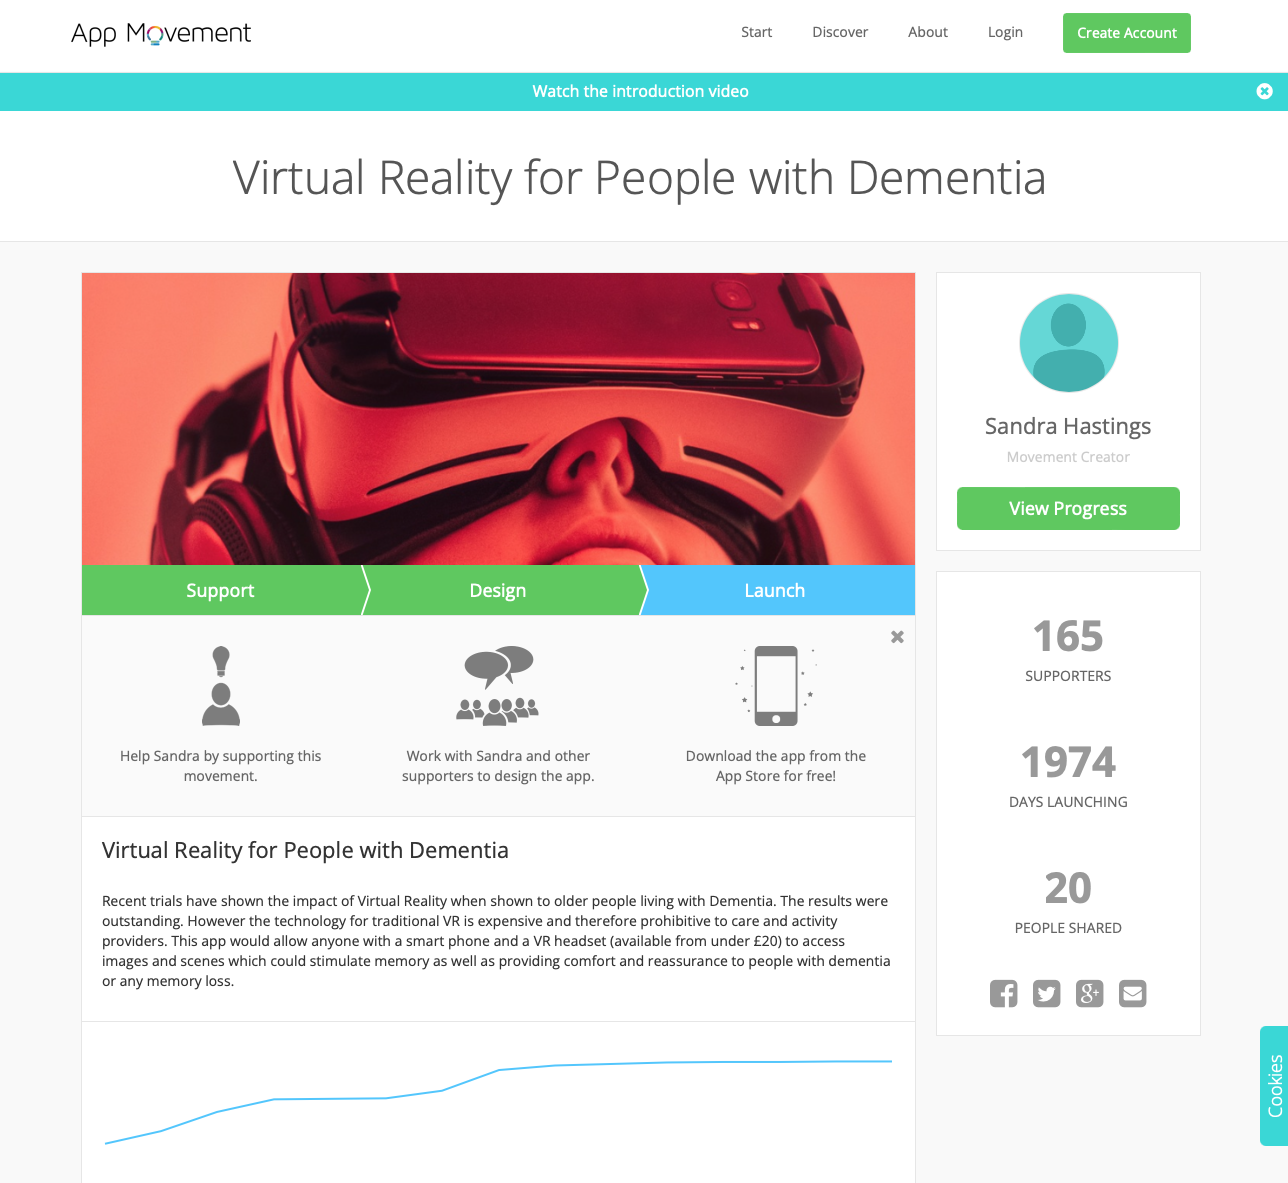
\includegraphics[width=0.6\linewidth]{Images/Methodology/AppMovement-SilverlineMemories.png}
    \caption{Silverline Memories post on App Movement designed by  \cite{garbett_app_2016} at Open Lab, Newcastle}
    \label{fig:AppMovement-Sandra}
\end{figure}

For the initial  stages of the thesis, I worked with Silverline Memories, a local registered charity in Newcastle upon Tyne, UK. The charity prides itself on activities for people with dementia, day trips out, celebrations for members' birthdays and other special occasions. During my time with Silverline Memories, I worked closely with the CEO, Sandra, who initially expressed interest in VR experiences in 2016 when she submitted a post on App Movement (see fig.\ref{fig:AppMovement-Sandra}), a community commissioning platform that enables users to ``collaborate, design, and deploy...a mobile application'' \citep{garbett_app_2016}. Due to the platform being limited to a set of app templates, the design of a VR app was not possible. Alternatively, given my interest in VR and dementia, I was able to provide an exploration and support into how Silverline Memories members could use VR. 

The relationship and involvement of Silverline Memories span across the first two chapters that primarily focus on the design of VR and media experiences for families with dementia. Working with the charity provided access to a larger group of people with dementia and their care partners than I initially anticipated, as prior work suggests difficulties in recruitment. However, working with a limited geographical area and recruiting through a gatekeeper did cause several issues. 

For instance, the members involved in the studies come from a white working-class demographic and predominately grew up in Newcastle, which presents a similar upbringing and lifestyle of living with dementia in the participants I recruited. As such, throughout the PhD, I worked with multiple different people with dementia from all stages of dementia rather than being able to focus on the early or advanced stages of dementia. Instead of offering interest to all the members at Silverline Memories in the studies, Sandra carefully selected members for me to talk to and recruit. Sandra's long-term relationships with the members saved time in recruiting and building the researcher-participant relationship phase. However,  it limited the study to some extent, in which I was not able to recruit based on needs or backgrounds.

\subsection{Recruiting online}
\label{Method:RecruitOnline}
In the final study, I could no longer work with Silverline Memories due to the pandemic. While the charity supported various online Zoom activities during COVID, most attendees were care partners. The current members were primarily in the later stages of dementia and rarely interacted with the online sessions. Instead, I branched out to contact multiple dementia advocate groups who had continued to share their stories and raise awareness online. For example, I reached out to the 3 Nations Dementia Working Group. They shared the recruitment poster in their online bulletin and gained interest from several steering group members. From reaching out to several groups and dementia advocates, only five people with dementia participated in the study in chapter seven. While the stages of dementia range from early to late, all the participants held a conversation and had strong verbal abilities to engage over Zoom meaningfully. In contrast, the studies in chapter four draw attention to the potential ways of participating through expressing themselves through gestures, laughing and movement that significantly support non-verbal communication.

\subsection{Reflections on recruitment}
As suggested by multiple researchers in dementia, recruitment often comes with multiple challenges, particularly at later stages of dementia, who are often more under-represented than in other stages of dementia \citep{bartlett2019strategies}. Working with the groups that I did in the North East, participants were predominantly from a working-class background who often had their spouse as a care partner. Meanwhile, the participants I worked in the study described in chapter seven came from mixed backgrounds, such as an accountant, human rights lawyer, and social worker. 

However, one limiting factor in the sampling and in many dementia works is that many groups are further underrepresented, such as the LGBTQ+ community, cultural diversity, young onset dementia, and advanced dementia \citep{mcgovern2014forgotten}. In one of my interviews with Howard from chapter seven, he described that while their working group has \textit{``started to get people from ethnic, LGBTQ+ backgrounds, it is still far from being done...''}. As such, while the work has involved a variety of diverse backgrounds, they are groups that are yet to be integrated into research recruitment pools and dementia networks and activity centres. 

\section{Data Collection}
\label{Method:DataCollection}
I collected data through various technologies and techniques throughout the PhD seen in table \ref{tab:OverviewDataCollection}. As I continued to learn from my successes and mistakes, the data collection evolved throughout the research. While I detail the data collection and treatments in their associated chapters, it is worth presenting an overview of the four phases of data collection, the type of data I collected, and how I prepared the data for analysis. For an example of the official university data management procedure, see appendix \ref{app:DataManagement}.

% Please add the following required packages to your document preamble:
% \usepackage{graphicx}
\begin{table}[htp]
\centering
\caption{Overview of collected data}
\label{tab:OverviewDataCollection}
\resizebox{\columnwidth}{!}{%
\begin{tabular}{l|llllll}
\textbf{} &
  \textbf{Interviews} &
  \textbf{No. Workshops} &
  \textbf{\shortstack{Field Notes \\ (words)}} &
  \textbf{Photography} &
  \textbf{\begin{tabular}[c]{@{}l@{}}\shortstack{Video/Audio \\ (mins)}\end{tabular}} &
  \textbf{\shortstack{WhatsApp \\ (messages)}} \\ \hline \\
\textbf{Study One}   & x                 & 3 avg. 65 mins  & 20,000  & 447 & 660 & x                                      \\
\\ \textbf{Study Two}   & x                 & x                 & 11,355 & 130 & 157 & 270 \\
\\ \textbf{Study Three} & 22 (avg. 50 mins) & x                 & x       & x   & x   & x                                      \\
\\ \textbf{Study Four}  & 11 (avg. 77 mins) & 12 (avg. 63 mins) & x       & x   & x   & x                                     
\end{tabular}%
}
\end{table}

\subsection{Phase One - A Reflective account on sharing a virtual world with people with dementia}

A significant part of the thesis builds on two studies where I worked closely with a dementia café to explore virtual reality environments. Through these two studies, I began to understand the researcher's role in conducting studies, and the challenges of involving people with dementia that are highly social and politically complex. Furthermore, by working with family members, I realised many of these challenges should be tackled in a more multidimensional fashion by recognising and including multiple narratives about dementia. In that respect, phase one describes a reflective account to provide a clear account of my background, history, the perspective on dementia, and design approaches that ultimately impact the participants, the setting and the overarching work (see \ref{Method:Reflectivity} for more information about my reflexivity as an approach).

Through phase one (seen in chapter four), I provide insights into designing VR environments for families with dementia and a personal narrative, that recognises the concerns, dilemmas, and the impact of working within sensitive research spaces. The account draws from the two studies below consisting of: field notes, audio recordings, videos, and photography. 
\begin{itemize}
    \item \textbf{Study one:} In 2017, as part of my undergraduate dissertation, I worked closely with a local dementia café called Silverline Memories, which had expressed an interest in virtual reality in dementia. The primary aim of this project was to explore, via collaborative workshops, the type of virtual reality environments and interactions people with dementia may want. Through these interactions with seven participants, a secondary aim was to design personalised VR experiences for couples with dementia to understand how VR could provide aesthetically meaningful experiences. I published this paper at CHI'18 with the co-authors.

    \item \textbf{Study two:} In 2018, through the master's and first year of the PhD, I continued my collaboration with Silverline Memories to explore the opportunities and challenges of designing enriched personalised multimedia experiences with people with dementia and their families. Adopting walking interview approaches to support wellbeing and provide the family with dementia agency in the interview, I designed a set of days out with all three families to create enjoyable or memorable moments, which I then sought to capture and document with audio recording, 360-degree videos, and photography that followed with a series of workshops to consolidate the personalisation and to store of the created moments from their days out. I published this paper at CHI'19 with the co-authors. The combination of moments captured by the families and ideas from the workshops resulted in the first year of the PhD developing a set of' moment boxes' for the families consisting of dioramas; QR codes to access the 360-videos; VR tours of the days out; day out related sensory objects such as seashells, tree bark; and a set of edited photos of the families on their days out.

\end{itemize}

Through this chapter, I raise numerous questions about consent, ownership and the building of relationships through adapting participatory methods to my research. In response, the two chapters that proceed with this first data chapter respond to a) the shifting sensitivities designers and developers may have when learning about dementia, and b) the ethical concerns HCI researchers face in the dementia context.

\subsection{Phase Two - DemVR: A hackathon exploring public engagement with dementia}

Following phase one, which focused on tailoring the design of virtual and media experiences for families with dementia, at the time, local authorities across Newcastle were interested in broadening the work to the public through technology events - such as a hackathon. At the same time, the interest offered an opportunity to examine public perception and the ways storytelling from people with dementia can influence the design process. Design events such as hackathons \citep{olesen_what_2021}, design sprints and workshops, involving as they do interdisciplinary teams interested in innovation, have been said to \textit{``offer new opportunities and challenges for cooperative work by affording explicit, predictable, time-bounded spaces for interdependent work and access to new audiences of collaborators''} \citep{filippova_hacking_2017}. Originating within the tech industry as competitive over-night coding events \citep{jones_theres_2015}, hackathons are events where designers, and developers collaborate over a short intensive period (typically a weekend), on software or design projects \citep{nandi_hackathons_2016}. 

In 2019, I set up a design hackathon to invite designers, developers and people with dementia to develop prototypes of VR environments that encourage shared experiences between people with dementia and others. To provide people with dementia and care partners an opportunity to develop ideas, I planned and arranged a six-week pre-hackathon consultation period to be carried out via 1) an online participatory platform, and 2) in-person workshops with people with dementia and their care partners. I designed the two activities to support people with dementia to engage in design activities to illustrate their desired VR shared experiences and bridge the gap between designers, developers and people with dementia on the online platform. However, as I describe in chapter five, the attempts to involve people with dementia and their care partners were significantly limited to one care partner's involvement engaged through our online platform. Throughout the study, I gathered data in four different ways:
\begin{itemize}
    \item Text data from the online participatory platform, consisting of comments from participants and 11 submitted ideas
    \item Video and audio recordings of three keynotes, 15 minute Q\&A with a person with dementia, and teams' presentations from the two-day event.
    \item Images, audio recordings and text data from team WhatsApp groups show the team's design process.
    \item Observational field notes were taken throughout the event, highlighting conversations with teams and facilitators.
\end{itemize}

\subsection{Phase Three - semi-structured interviews with researchers to elucidate the ethical challenges in dementia co-design}

From phases one and two, the data collected presents insights into the challenges and opportunities researchers might encounter when involving people with dementia in the design process. While this provides initial findings into the ethical concerns in dementia and HCI, it does not provide an overarching understanding of the role of ethics in HCI and dementia. In 2019, I invited several dementia-HCI academics to collaborate on design ethics in dementia and HCI research, where we would reflect as a community of practice and elucidate broader concerns about ethics in HCI research.

The data consists of interviews with 22 self-identified designers and/or researchers who reported significant experience in working with people with dementia. Each participant was invited to a 45-60 minute interview which consisted of open-ended questions and prompts such as: 1) experience with institutional ethics processes, 2) technological ethics,
3) power relationships, and 4) research impact. Five of the authors conducted the interviews, which were carried out in person where possible, but otherwise carried out over video calls. With 1,100 minutes worth of interview data, UKTranscription transcribed the interviews, and I re-reviewed transcriptions to ensure anonymisation.


\subsection{Phase Four - Dialogical Dementia Design Toolkit: exploring the type of resources for educating designers and developers when designing for and with people with dementia}

During the final phase, I built upon the reflections of the hackathon, where it became apparent that interactions between those with dementia and others outside of the community remain sparse. The final study considers: how toolkits and other creativity support tools foster dialogical engagement between people with dementia and designers and developers? To explore the work area, I invited 11 self-identified designers/developers and five people with dementia to examine the type of resources developers and designers need to design with people with dementia and investigate how people with dementia envision their potential participation within a toolkit.

Due to conducting the study over the pandemic, the workshops and interviews were all online. They required inviting people with dementia who had access to the internet and had a reasonable function of their verbal communication. I collected the workshops and interviews via Zoom/Teams recordings. Group workshops with designers and developers and one-to-one interviews with people with dementia were split across three stages of data collection. Stages one and two focused on gathering data to develop the dementia design toolkit incrementally. For the third stage, I presented the toolkit to participants to gather feedback and critique in its roughly 'final' stage. Zoom was chosen for the interviews as the participants with dementia preferred it. Designers and developers joined a scheduled Teams meeting for the workshops, with additional activities on a shared online whiteboard space (a Miro board).

For preparing the data, I initially used two auto-transcription tools to speed up the transcription phase. This was due to the first two stages of the design process requiring a quick and iterative process for the affinity diagramming, which helped shape the early design rationales and initial toolkit components. For the designer and developer workshops, I used the Microsoft Team's built-in recording and transcription tool that Newcastle University supports. In contrast, given the data sensitivity for the interviews with people with dementia, I used the Google Pixel on-device Audio recorder that supports offline text to speech translation. This was due to privacy issues regarding Zoom and Otter.ai that reuse data to improve their AI model accuracy. Following the auto-transcription process, I revised the transcriptions for any misinterpretations and added any necessary anonymisation. 

\section{Qualitative data analysis}
\label{QualDataAnalysis}
We see the use of qualitative research more regularly in dementia research. The approach allows the researcher to build a complex understanding of people with dementia in everyday experiences \citep{mckeown_actively_2009}. Thematic Analysis (TA), which I primarily used to analyse the collected data, is a popular approach to qualitative data to examine common connections between datasets. TA is the process of \textit{``identifying, analysing, and reporting patterns (themes) within data''} \citep{braun_using_2006}. Given the rich descriptive data I collected through the PhD, TA provides an analysis ``that reduces the data in a flexible way that dovetails with other data analysis methods''. \citep{kiger2020thematic} suggest that thematic analysis is a proven approach that works well for providing highly descriptive and conceptual findings in their results. As thematic analysis provides steps to organise the data through labels and themes, the process provides transformative approaches to understanding the meanings and experiences of the participants within the data. Further, \cite{braun2012thematic} emphasise that researchers should draw attention to the actual process researchers undertake to ensure confidence in the findings. As such, I describe the TA process I followed below.

The thematic analysis approach I followed was in line with the instructions set out by \cite{braun_one_2020}. This process consists of seven steps: 1) preparing data through transcripts and additional data cleaning; 2) familiarising myself with the data while referring to the research questions. Following, structure the data in a way to make sense of the similar conversations between participants; 3) move onto the coding process to identify all relevant data by line-by-line coding, tagging and highlighting anything of interest; 4) organise codes into potential linking themes; 5) reviewing themes; 6) discuss the initial themes with supervisors to see if they fit with the original research questions and name the themes. Finally, step 7) is to finalise the analysis by writing and presenting it in the data chapters. Data was collected and analysed chronologically to the chapters that are set out in the thesis. An example can be found in the appendix \ref{app:TA}.


In \cite{braun_one_2020} recent work on TA, the authors reflect on the challenges regarding how their work in 2006 did not intend to be a one-size fits all approach \citep{braun_using_2006}. Instead, the authors refer to TA as \textit{``rather a cluster of sometimes conflicting approaches, divergent both in procedure and underlying philosophy, but which share an interest in capturing patterns in data''} \citep[pg.333]{braun_one_2020}. As such, they suggest TA should embrace the flexibility that the method brings to qualitative research, which must also consider the skills and values the researcher brings to the process. Through the social constructionist approach I adopt, my epistemology has significant implications for the thematic analysis approach regarding identifying themes that represent meaning or meaningfulness to the topic instead of the recurrence within the data.

\subsection{Validity and reliability in research}
\label{TA:Reliability}
One of the biggest challenges qualitative researchers undertake is assuring their research is trustworthy and rigorous \citep{finlay2006rigour}. These challenges are criticised for being ambiguous in the researcher's analytical processes, findings being a collection of opinions subject to research bias, and poor justification of the methods adopted \citep{rolfe2006validity}. Typically, reliability, validity, and generalisability concepts provide a framework for evaluating and conducting quantitative research. However, whether these terms are appropriate for qualitative research is continuously debated among academic researchers, given how inherently different qualitative research is from quantitative \citep{ryan2009rigour}. Alternatively, \cite{noble2015issues} propose a set of strategies to ensure trustworthiness in qualitative research:

\begin{center}
\begin{tabular}{ | m{17em} | m{17em}|  } 
  \hline
  \textbf{Proposed Strategies} & \textbf{How I implemented the strategy}  \\ 
  \hline
   Meticulous record keeping, demonstrating a clear decision trail and ensuring interpretations of data are consistent and transparent.
  &  Through the PhD, I have kept a reflexive journal that provided a map of my thoughts and study process. This reflexive journal as described in \ref{Method:Reflectivity}, has been a useful guide in conducting my analysis on the Thesis data.
 \\ 
 \hline
 Accounting for personal biases, which may have been influenced by the findings. 
  & As well as keeping a reflexive journal, the following chapter is a reflective account of my first two studies in dementia-HCI research that reflects on the type of researcher I am. \\ 
  \hline
   Including rich and thick verbatim descriptions of participants’ accounts to support findings.
  & The findings found in each data chapter are rich with participant's quotes that are representative of what they said during the study.  \\ 
  \hline
   Engaging with other researchers to reduce research bias.
  & While the thesis is primarily my work, I have collaborated with several researchers as well as with my supervisors to ensure the analytical process represents the research questions.  \\ 
  \hline
   Respondent validation: includes inviting participants to comment on the interview transcript and whether the final themes and concepts created adequately reflect the phenomena being investigated.
  & In chapter \ref{D3}, I sent participants a list of quotes and associated theme names to double-check that I accurately represented their data in the analysis. \\ 
  \hline
   Data triangulation, whereby different methods and perspectives help produce a more comprehensive set of findings.
  & As described in the data collection section (\ref{Method:DataCollection}), Most of the thesis consists of multiple sets of data collection that provided multiple different perspectives and viewpoints to be shared through this work.  \\ 
  \hline
  
\end{tabular}
\end{center}

Although there is no one-size-fits-all approach to providing trustworthiness in qualitative research, embracing some of the strategies above will provide work that is more mindful of the assumptions and methodological choices made within the researcher's work.  


\section{Reflexivity}
\label{Method:Reflectivity}
Although chapter four acts as a reflective piece that \textit{``acknowledge[s] the multiple roles, identities and positions that researchers and research participants bring to the research process''} \citep[pg.395]{milner2007race}, it is worth examining and reflecting on the way I view the world and the personal understanding of my role as a researcher as the thesis progressed. From early on, it was very apparent that my experiences during and outside the studies would influence the interpretations I made through my analysis. As such, \cite{probst2015eye} describes reflexivity as:
\begin{quote}
\textit{``Despite its "messiness," reflexivity remains a fundamental way, particularly in qualitative studies, to bolster credibility by parsing the research endeavor into its mutually affecting parts and documenting the pathways through which knowledge was generated.'' \citep{probst2015eye}
}\end{quote}

Reflexivity offers a critical way to stay self-aware through the thesis. Still, more importantly, it is a way to acknowledge the emotional and often challenging experiences that a researcher may encounter when working within sensitive settings - like dementia. \cite{corlett2018reflexivity} recognises reflexivity offers readers insight into the researcher's motivations and interests, which is crucial because research is \textit{``as much the researcher's story as it is the story of [the] participants''}. Furthermore, this reflective practice plays a critical role in the thematic analysis to understand the different roles and identities between the stakeholders and myself. \cite{day2012reflexive} pays further attention to recognising the emotional labour in conducting research and how it is an integral part of research data. Day pulls from Hoffman's work and characterises that emotional labour \textit{``shifts the power relationship between interviewer and [participant]''} where the researcher and participant produce a shared knowledge about the research. To unpack my reflections, I first describe my positionality, followed by a reflective piece from my field notes highlighting the personal development of becoming a researcher.

\subsection{Positionality}
\label{Method:Positionality}
I received my undergraduate in computer science (CS), where the modules prioritised software engineering skills such as coding best practices, databases, and back-end and front-end web technologies. Until the third year, the course taught very little about Human-Computer Interaction. In the third year dissertation, I went on to work in Open Lab where I explored the role of VR for people with dementia. While the VR interest was due to the novelty and recent excitement in the media, the dementia thread is tied to family experiences where my Grandpa lived with dementia. Consequently, as I describe in chapter four, how my Grandma delivered care and described dementia significantly influenced my perspective and expectation of working with dementia. 

Following my undergraduate, I joined Open Lab, Newcastle University as a PhD candidate as part of their centre for doctoral training in Digital Civics. The four-year programme combines a Masters of Research (MRes) in Digital Civics and a three-year funded PhD. As part of the doctoral training, each year, Open Lab enrolled a set of ten students through a cohort approach that consists of diverse interdisciplinary skills and backgrounds. Coming from a computer science background, the design and critical thinking required for HCI was a skillset that was untaught and needed continuous adjustment and learning through reading and integrating the learnings into practice. For example, my early work was more technically focused through an emphasis on `techno-fixing' where I envisioned technology could provide a solution to societal problems \citep{jongsma2017usual}. However, over time as the thesis demonstrates, the focus shifted toward understanding the ethical complexities of adding technology to an already complex and sensitive setting and how technology might fit the needs of the person with dementia.

\subsection{The researcher's role}
\label{Reflexivity:Questions}
Throughout the PhD, I have made many relationships with participants I still talk to after finishing the study. For instance, Jim, a participant in my final study, will still email or occasionally video call to chat about dementia activist topics and general day-to-day conversations. This is often due to my early recruitment stages requiring openness from myself to get to know the participant and make them feel comfortable in my presence. Typically, participants would often ask \textit{``why are you looking into dementia?''} Looking back at my reflexive journal - that researchers recommend for during the research process and coding stages, I found this excerpt from  replying to the question above:

\begin{quote}
 \textit{   
\textbf{James}: ``Well, I'm not sure if you remember, but last year [2017] I worked with a couple of you to create some VR experiences that looked at ways to personalise the environments for members here [ at Silverline]. As I got to know the area more, I talked to my Grandma about my research. One of the reasons I thought about dementia research was because of her. My Grandpa had Alzheimer's in his early 50's. He sadly passed away when I was five… Of course, I didn't get to know him that well, but through the circumstances my Grandma shares stories of him. She shared stories of before the diagnosis and many that of her relationship with him after his diagnosis too.''}\par


\textit{\textbf{Kate}: ``are you close with your Grandma?''
}\par


\textit{\textbf{James}: ``Very much so... I call her every few days and we talk about all sorts… To me, It's been interesting to hear my Grandma's side towards caring for my Grandpa too. The stories of her having to learn how to organise the bills, or mortgage – she had to take on so many social roles that he once proudly had… But also, she told me when she told him to get off his back-side and stop feeling sorry for himself… She would make alternations around the house to ensure he could do many of the roles he once felt like he lost – at least to the extent that he thought he could see fit.''}
\end{quote}

\textbf{My reflexive journal comment: 
}
\begin{quote}
\textit{``As I began to share stories of my family, Kate started to cry. Kate shared how much the story reflected her experiences too. We started to share stories from each family side. Kate had gone through similarities to my Grandma with having to change significant social and, even in their eyes, gender roles. I feel perhaps Kate and I have bonded over these stories. Maybe she trusts me more now she knows why I care for making some change in dementia? We both cried, laughed and smiled, listening to each other's stories. It felt strange to me that this felt so wrong. A relatively common interaction among friends, maybe not so much between somewhat strangers, but what made me feel 'wrong' was that my openness made me assume I was a bad researcher.''}
\end{quote}

Although the reflective texts in my journal are not part of the data I analysed, they helped with the personal development of my role as a researcher. Throughout the thesis, I was aware that by working with people with dementia and having families ties to the condition, the stories participants shared would impact me in ways beyond the academic day-to-day. During my time conducting this research, I distinctly remember questioning \textit{`how is my research helping dementia?'} and \textit{`what is even the role of me, the researcher, in this work?'} As I describe in the reflexive journal, at the time, I felt guilty of sharing personal stories and thought I might be contributing to an emotional burden through sharing rather than \textit{`making things better'}. However, over time, I realised that emotional work is expected in this type of research, and that is okay. 

At the start of 2020, I received the news that Dorothy, who showed so much enthusiasm and joy for the Shania Twain VR concert hall I created (in my undergraduate), had sadly passed away. Dorothy and I never verbally communicated. Yet, I still remember all these years later the first time she smiled and started to hum along to 'You're Still the One' by Shania Twain. I'm not sure if that moment or myself stuck with Dorothy afterwards. However, I learned something significant in that interaction, at the very least. I learned that part of research is about accepting and reflecting on those emotions and experiences researchers have within this sensitive type of work. It is not as simple as collecting a set of stories and writing an analysis about their lives. Instead, researchers are part of that experience. While I learned a lot of unique insights into dementia through this PhD, I also have learned many life lessons that influence who I am today. For that, I am very grateful to my participants for willingly sharing their stories and wisdom.

\section{Summary}
\label{Method:summary}
This chapter gives a detailed overview of the research approach I undertook to explore the research questions I set out in the introduction. At the start of this chapter, I describe how researchers have adapted participatory methods to fit the needs of people with dementia, including the ethical considerations required when working in sensitive settings. I then introduced descriptions of the data collection within each data chapter that are described in more detail in their corresponding chapters. To conclude the methodology chapter, I detail the data analysis process I used to make sense of each chapter's data. Subsections further support this on reflexivity, validity, and reliability of research. To conclude this chapter, it is worth revisiting the research questions in response to the methodologies outlined in this chapter.

% Please add the following required packages to your document preamble:
% \usepackage{graphicx}
\begin{table}[htp]
\caption{Research questions and methodological approaches}
\label{tab:RQ-Methods}
\resizebox{\columnwidth}{!}{%
\begin{tabular}{l|ll}
\textbf{Research questions} &
  \textbf{Methodological approach} &
   \\ \cline{1-2} \\
\textit{\begin{tabular}[c]{@{}l@{}}How might participation \\ be configured for people \\ with dementia to shape the \\ design process of technology?\end{tabular}} &
  \begin{tabular}[c]{@{}l@{}}Through the collection of field notes, videos, \\ audio, and workshops, I explore ways walking\\  interviews (\ref{PD:Interviews}), and online platforms (\ref{PD:onlinePlatform}), \\ might be configured to shape the design process \\ for people with dementia.\end{tabular} &
   \\ \\
\textit{\begin{tabular}[c]{@{}l@{}}What are the ethical implications \\ for people with dementia to \\ participate in HCI research?\end{tabular}} &
  \begin{tabular}[c]{@{}l@{}}Collection of reflexive data concerning my \\ engagement with families with dementia - presenting \\ a series of potential implications of dementia (chapter four). Later \\ in the thesis, given that researchers/designers are \\ designing participatory and co-design processes for people \\ with dementia, collecting a series of interviews with HCI\\ designers/researchers and analysing the data provides \\ unique findings and directions within everyday interactions \\ with people with dementia (chapter six).\end{tabular} &
   \\ \\
\textit{\begin{tabular}[c]{@{}l@{}}What are the competing interests \\ and expectations to support \\ meaningful dialogue in dementia \\ design research when involving \\ multiple stakeholders - such \\ as people with dementia, \\ developers, designers and \\ researchers?\end{tabular}} &
  \begin{tabular}[c]{@{}l@{}}By inviting a diverse set of stakeholders through the thesis, \\ the overarching analysis provides insights into the interests and \\ expectations of people with dementia, family members, \\ researchers, designers and developers. Chapter seven uses \\ an iterative design process through interactive workshops\\ and interviews to design the type of resources developers \\ and designers need to design with people with dementia \\ and investigate how people with dementia envision their \\ potential participation within a toolkit. \end{tabular} &
  
\end{tabular}%
}
\end{table}